\documentclass[12pt,twoside,a4paper]{article}

\usepackage[margin=2cm]{geometry}
\usepackage[slantfont,boldfont]{xeCJK}
\usepackage[utf8]{inputenc}
\usepackage{listings}
\usepackage{float}
\usepackage{color}
\usepackage{xcolor}
\usepackage{caption}
\usepackage{color}
\usepackage{courier}

\definecolor{codegreen}{rgb}{0,0.6,0}
\definecolor{codepurple}{rgb}{0.58,0,0.82}
\definecolor{backcolour}{rgb}{0.95,0.95,0.92}
\definecolor{darkgray}{rgb}{0.3,0.3,0.3}

\newcommand{\inlinecode}[1]{\colorbox{backcolour}{\color{darkgray}\texttt{#1}}}

\DeclareCaptionFont{white}{\color{white}}
\DeclareCaptionFormat{listing}{\colorbox{gray}{\parbox{\textwidth}{#1#2#3}}}
\captionsetup[lstlisting]{format=listing,labelfont=white,textfont=white}
\lstset{
	backgroundcolor=\color{backcolour},
	commentstyle=\color{codegreen},
    keywordstyle=\color{violet},
    stringstyle=\color{codepurple},
	language=Python,
	numbers=left,
	numberstyle=\small\color{lightgray},
	columns=fullflexible,
	showstringspaces=false,
	breaklines=true
}

\setCJKmainfont{PingFang TC}

\title{CV HW2 Report}
\author{林義聖\\B03902048}
\date{}

\usepackage{graphicx}
\graphicspath{ {./} }

\begin{document}

\maketitle

\section{Introduction}

I use \textit{Python} as my programming language and \textit{Pillow} as my Image Library. Also, I use \textit{matplotlib} as the auxiliary program to draw the histogram from the data.

\begin{figure}[H]
\centering
\includegraphics[scale=0.4]{lena.bmp}
\caption{original lena picture}
\label{fig:lena.bmp}
\end{figure}

\section{Binarized the Image}
I use the following steps to binarize \textit{lena.bmp} with threshold set to 128.
\begin{enumerate}
	\item Read lena.bmp in as Python \textit{list}.
	\item For every pixels, compare its intensity to the threshold.
	\item if its intensity is higher, draw it as white, else draw it as black.
\end{enumerate}
\begin{lstlisting}[caption=Binarize the image]
threshold = 127
black, white = 0, 255
for i in range(height * width):
    output_data[i] = white if pixel_data[i] > threshold else black
\end{lstlisting}

\begin{figure}[H]
\centering
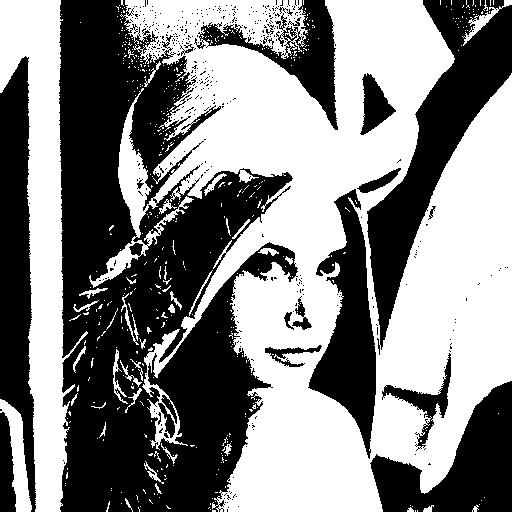
\includegraphics[scale=0.4]{lena-binarized.bmp}
\caption{binarized lena picture}
\label{fig:lena-binarized.bmp}
\end{figure}

\section{Draw the Histogram}
I use the following steps to calculate the histogram of \textit{lena.bmp}.
\begin{enumerate}
	\item Read lena.bmp in as Python \textit{list}.
	\item For every pixels, accumulate its intensity.
	\item Call \textit{matplotlib.pyplot.bar} to draw the histogram.
\end{enumerate}
\begin{lstlisting}[caption=Accumulating the intensity]
histo_data = [0] * 255
for i in range(height * width):
    histo_data[ pixel_data[i] ] += 1
\end{lstlisting}

\begin{figure}[H]
\centering
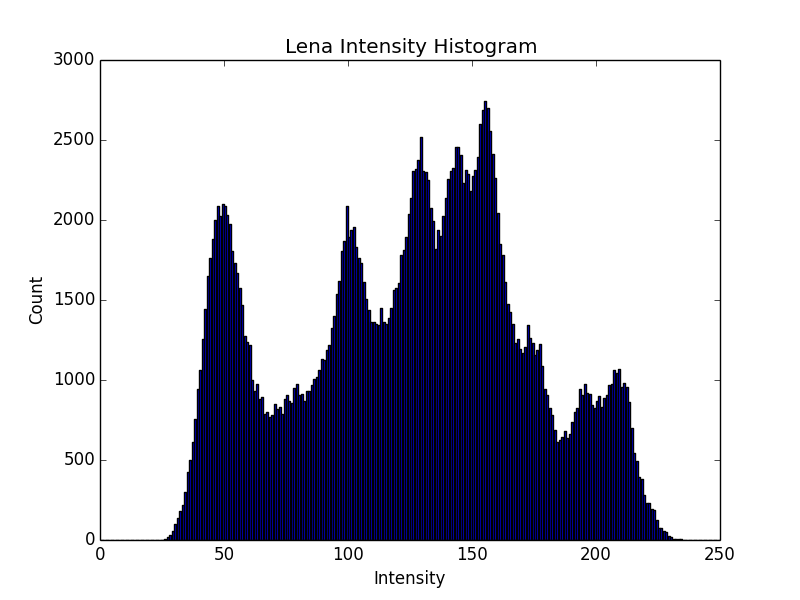
\includegraphics[scale=0.5]{lena-histogram.png}
\caption{histogram of lena picture}
\label{fig:lena-histogram.png}
\end{figure}

\section{Finding the Connected Components}
I use the following steps to find the connected components and draw bounding box on the picture.
\begin{enumerate}
	\item Take lena-binarized.bmp as input image, and read it in as Python \textit{list}.
	\item For every pixels (actually, only white pixel), give it a label first, then use \textit{BFS} to expand all connected pixels around it (8-connected).
	\item Count the numbers of pixels of each labels.
	\item Draw the bounding box (using function \textit{PIL.ImageDraw.draw.rectangle} to draw rectangles on output picture) around the group of connected components with size larger than 500.
\end{enumerate}

\begin{lstlisting}[caption=Finding connected components]
# 8-connected neighbor
nei_offset = [(-1,-1),(0,-1),(1,-1),(-1,0),(0,1),(-1,1),(1,0),(1,1)]
for y in range(height):
    for x in range(width):
        if label_map[y*width+x] == 0 and data_seq[y*width+x] == 255:
            curr_label = get_label() # assign a new label
            curr_color = data_seq[y*width+x]

            state_q = []
            label_map[y * width + x] = -1 # assign a temporary label
            state_q.append((x,y)) # push into state queue

            while len(state_q) != 0:
                tmp_x, tmp_y = state_q.pop(0) # pop out from queue and assign label
                label_map[tmp_y * width + tmp_x] = curr_label

                for offset in nei_offset:
                    off_x = tmp_x + offset[0]
                    off_y = tmp_y + offset[1]
                    if 0 <= off_x < width and 0 <= off_y < height and \
                    	label_map[off_y*width+off_x] == 0 and \
                    	data_seq[off_y*width+off_x] == curr_color:
                        label_map[off_y * width + off_x] = -1
                        state_q.append((off_x,off_y)) # push into state queue
\end{lstlisting}

\begin{lstlisting}[caption=Drawing the bounding box]
for i in range(1, len(count_label)):
    if count_label[i] >= THRESHOLD:
        # finding the boundary of the area of this label
        topVal = min(label_array[i], key=lambda x: x[1])[1]
        bottomVal = max(label_array[i], key=lambda x: x[1])[1]
        leftVal = min(label_array[i], key=lambda x: x[0])[0]
        rightVal = max(label_array[i], key=lambda x: x[0])[0]
        
        # draw bounding box and centroid with ImageDraw class
        sum_x, sum_y = 0, 0
        for j in range(len(label_array[i])):
            sum_x += label_array[i][j][0]
            sum_y += label_array[i][j][1]
        avg_x = int(sum_x / len(label_array[i]))
        avg_y = int(sum_y / len(label_array[i]))
        rcolor = (255, 0, 0)
        draw.rectangle([(leftVal,topVal),(rightVal,bottomVal)], outline=rcolor)
        draw.line([(avg_x-5,avg_y-5),(avg_x+5,avg_y+5)], fill=rcolor)
        draw.line([(avg_x+5,avg_y-5),(avg_x-5,avg_y+5)], fill=rcolor)
\end{lstlisting}

\begin{figure}[H]
\centering
\includegraphics[scale=0.55]{lena-bounding.bmp}
\caption{lena picture with bounding box}
\label{fig:lena-bounding.bmp}
\end{figure}

\section{How to Use}
There are three programs in my HW2.
\begin{enumerate}
	\item \textit{binarize-128.py}
	\item \textit{calc-histogram.py}
	\item \textit{find-connected-components.py}
\end{enumerate}
You just need to enter command in this format: "\textit{program [input image name] [output image name]}" to use it. For example, \inlinecode{./binarize-128.py lena.bmp output.bmp}.

\end{document}
